\chapter{Sistema Proposto}\label{cap3}


Essa seção apresenta as etapas de desenvolvimento do sistema de recuperação de atas proposto, bem como o seu funcionamento geral, desde a preparação dos documentos até a entrega dos históricos de ocorrência ao usuário. Inicialmente serão descritos a seleção e pré-processamento das atas. Em seguida, será relatado como as técnicas de mineração de texto e recuperação de informação são utilizadas nesse trabalho.

A Figura \ref{fig:visao-geral} mostra a visão geral do sistema proposto cujo objetivo é permitir ao usuário consultar uma coleção de documentos de reuniões a fim de obter todo o histórico de ocorrências de um determinado tema relacionado à pesquisa do usuário, podendo identificar nos documentos onde esse tema foi mencionado, bem como se houve uma decisão sobre o tema. Para isso, o sistema é divido em dois módulos principais: módulo de preparação e manutenção e módulo de consulta, os quais serão detalhados nas próximas seções.  % "isso envolve a classificação. Onde entram os tópicos?" --> Rafael

A Figura \ref{fig:visao-geral} mostra a visão geral do sistema com suas principais entradas e saídas. 


  %--- Figura Visão Geral ---
  \begin{figure}[!h]
	  \centering
	  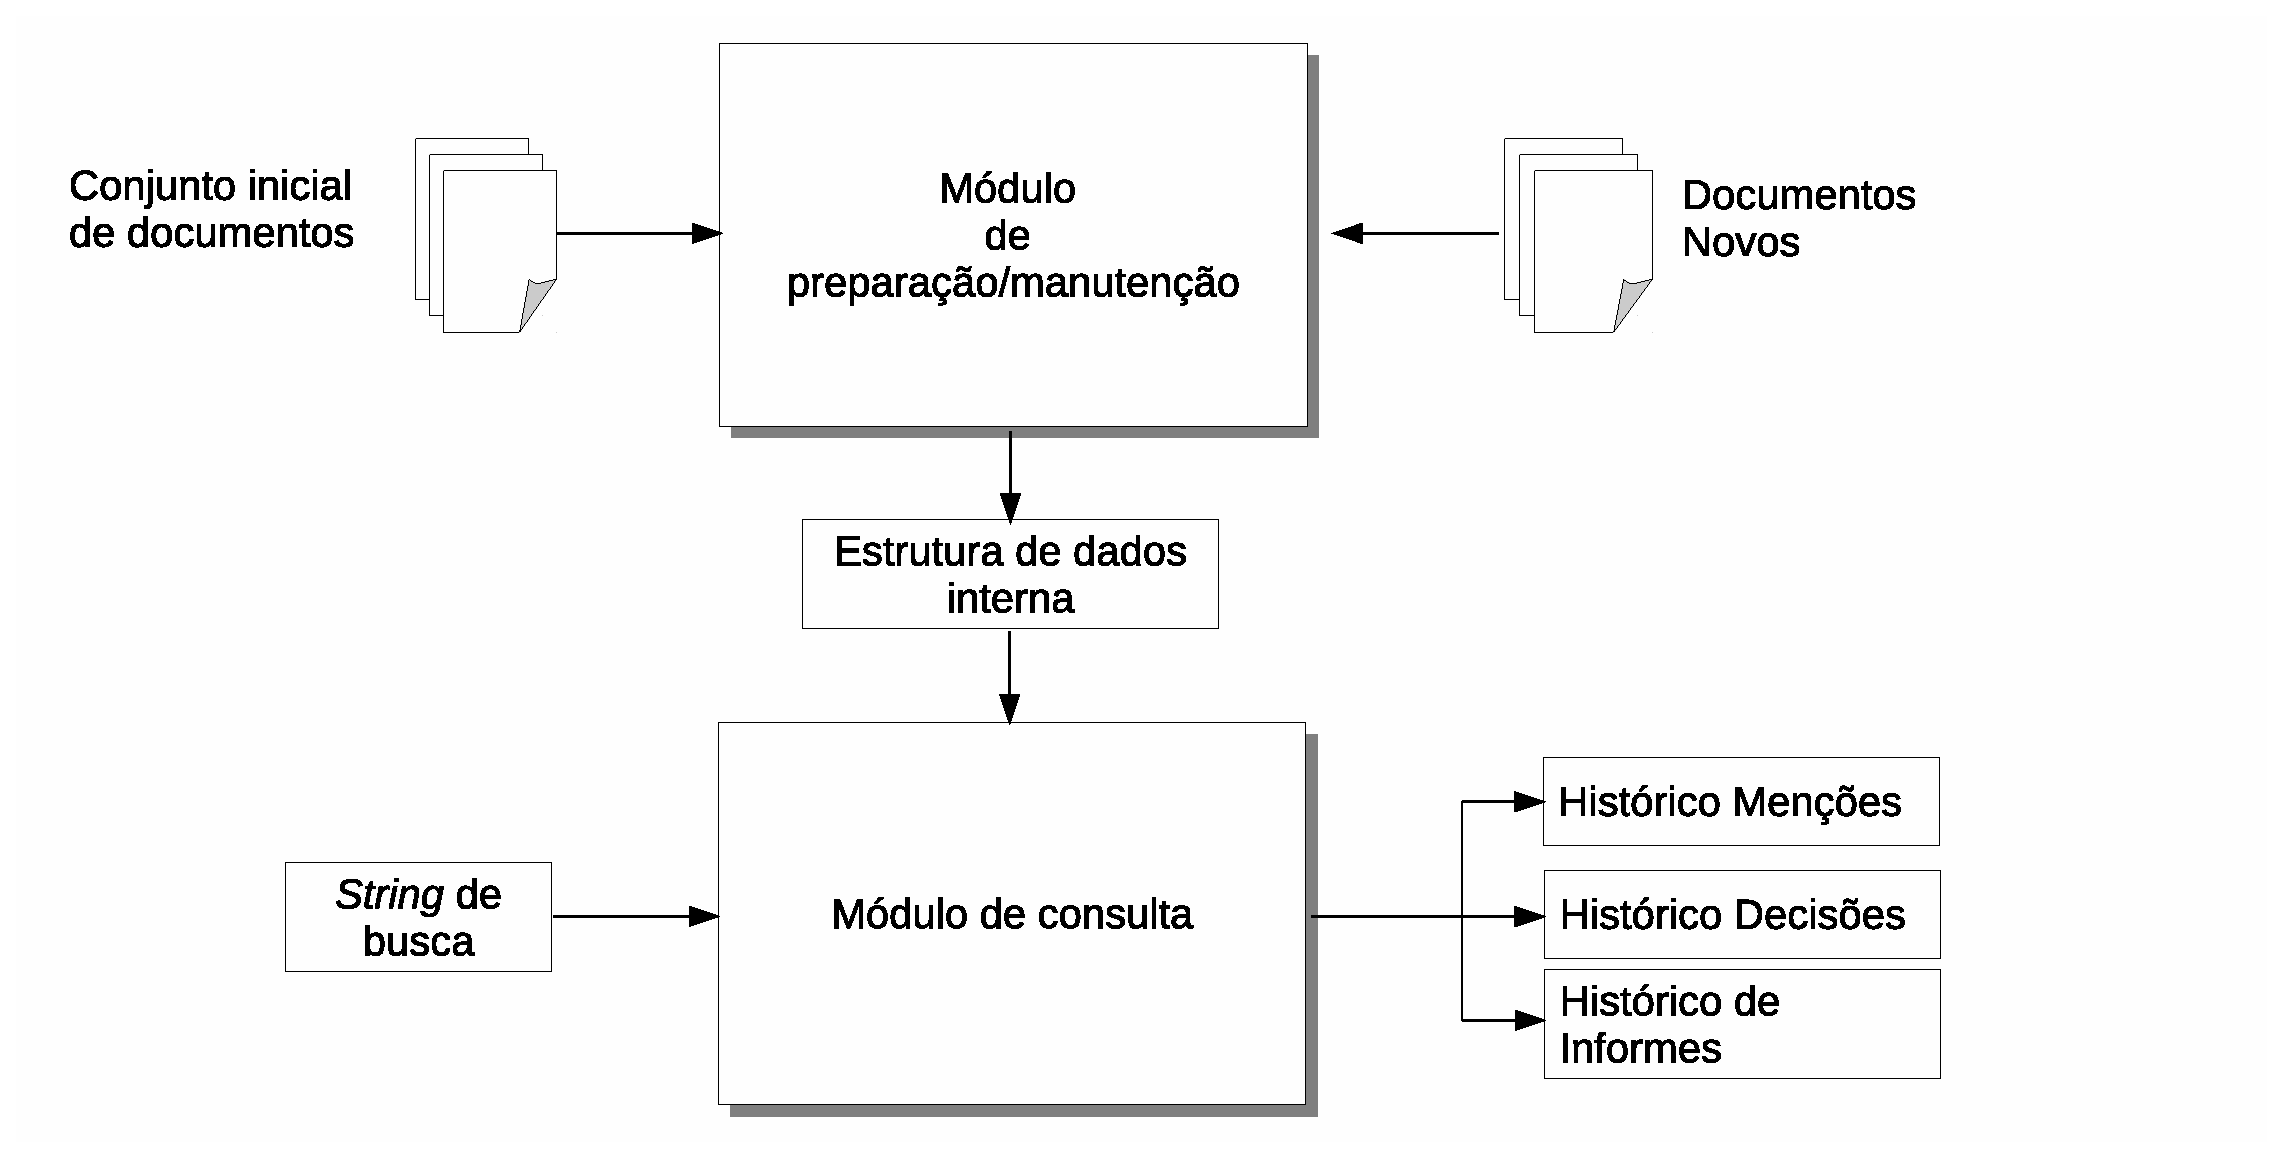
\includegraphics[width=0.69\paperwidth]{conteudo/capitulos/figs/visao-geral-3.eps}
	  \caption{Visão geral do sistema}
	  \label{fig:visao-geral}
  \end{figure}






\section{Módulo de preparação e manutenção}

O módulo de preparação e manutenção tem como funções principais dividir cada ata em em segmentos de texto que contêm um assunto predominante, e separá-los em categorias por meio de técnicas de extração tópicos e classificação. Além disso, produz uma estrutura de dados que registra quais assuntos foram tratados na reunião, bem como o trecho do documento onde é discutido.  
% melhorar ↓↓↓↓↓
% --> ↓↓  Texto introdutório  ↓↓
% --> ↓↓↓↓↓↓↓↓↓↓↓↓↓↓↓↓↓↓↓↓↓↓↓↓↓↓
A seguir são apresentadas as etapas do módulo de preparação e manutenção desde a preparação dos documentos até a entrega da estrutura interna ao módulo de consulta. 


\subsection{Preparação dos documentos}

As atas são normalmente armazenadas em arquivos binários do tipo \textit{pdf}, \textit{doc}, \textit{docx} ou \textit{odt}. As atas devem ser pré-processadas e estruturadas para que posam ser aplicados métodos de MI e RI. Inicialmente, o texto puro é extraído e passa por processos de transformação conforme apresentados a seguir.

A Figura~\ref{fig:exemplopreprocessamento} mostra a etapa de preparação de um documento em português que inclui a remoção de elementos menos significativos e a identificação de sentenças e segmentos.
	
% -<? Colocar aqui uma explicação do que é um segmento e uma sentença?

\begin{center}
	\begin{figure}

	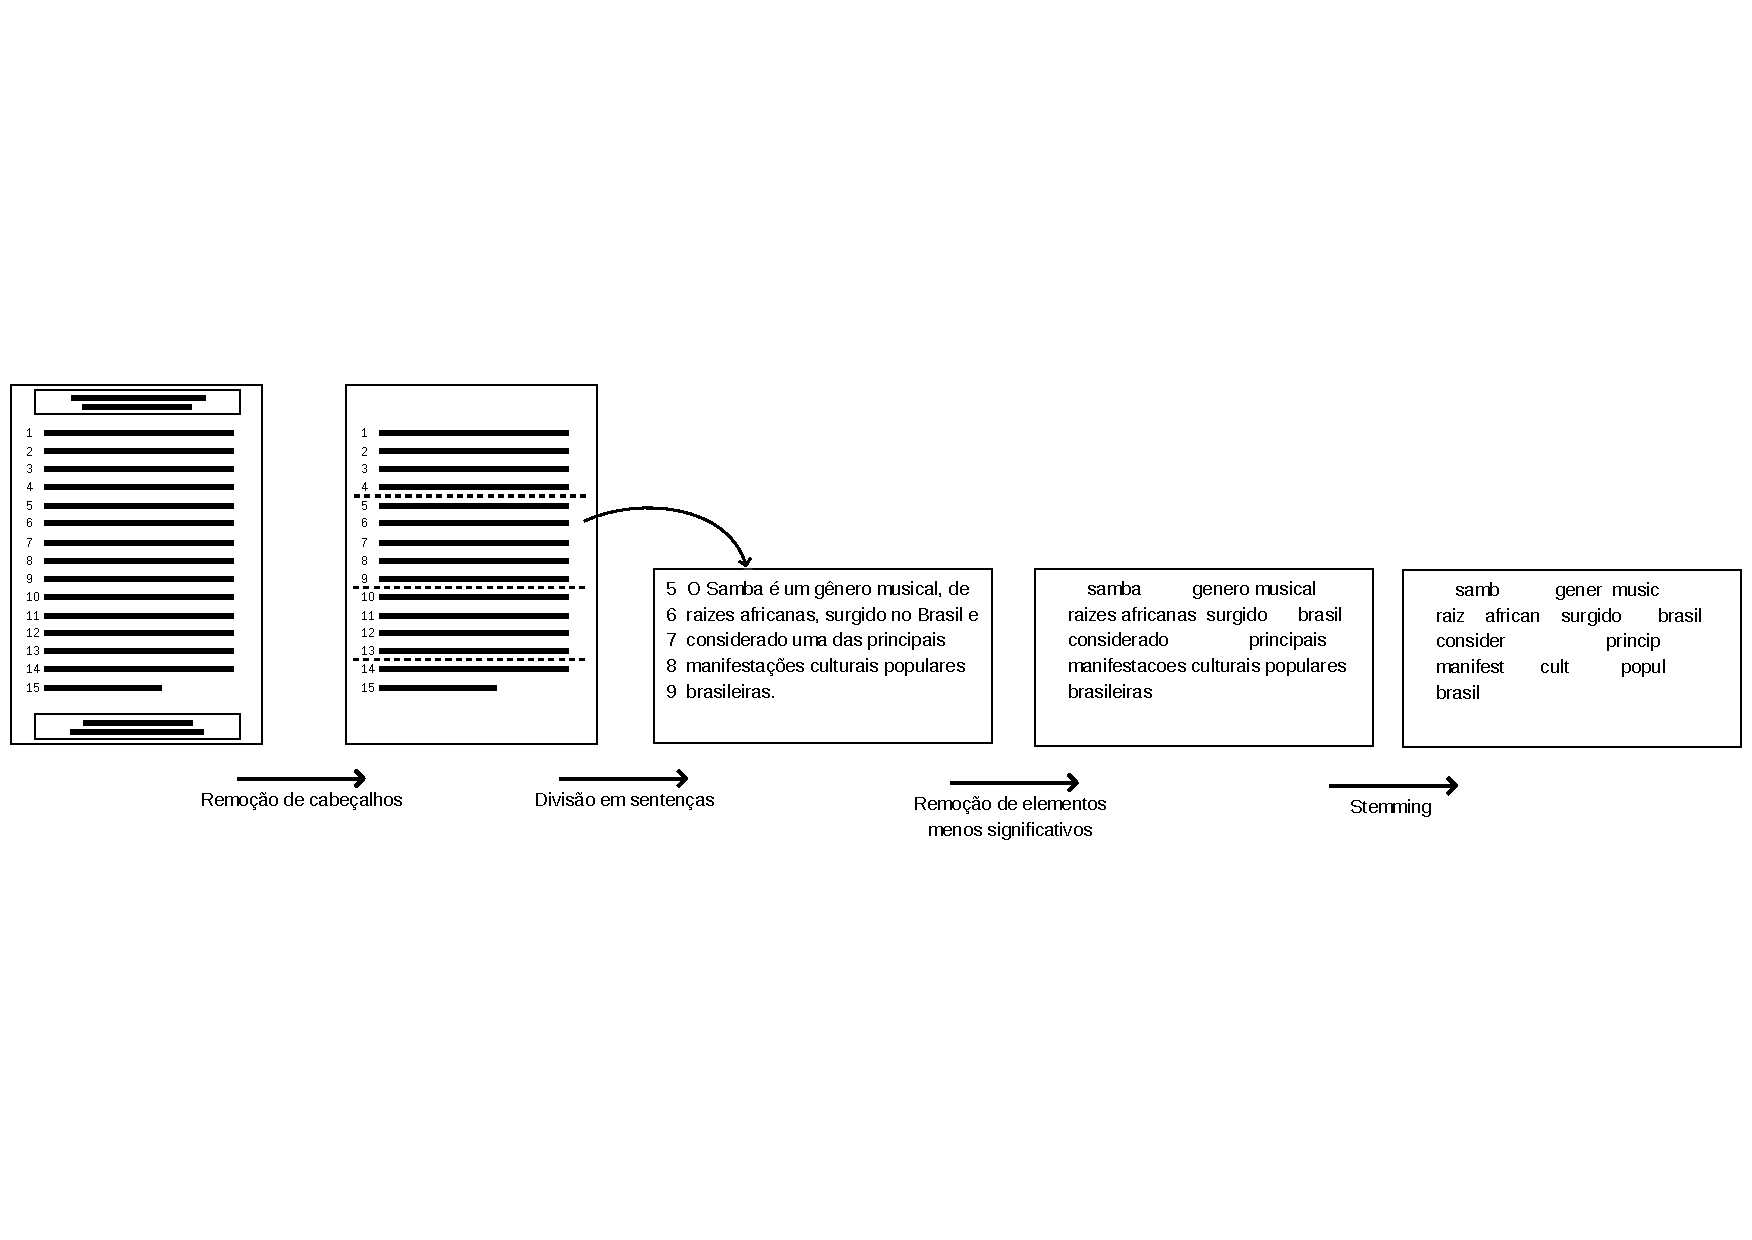
\includegraphics[trim={ 0 180 0 180 },clip,page=1,width=\textwidth]{conteudo/capitulos/figs/pre-process.pdf}

	\caption{Etapa de pré-processamento}
	\label{fig:exemplopreprocessamento}
	\end{figure}
\end{center}






\begin{enumerate}

%  Cabeçalhos e rodapés
\item Remoção de cabeçalhos e rodapés: as atas contém trechos que podem ser considerados pouco informativos e descartados durante o pré-processamento, como cabeçalhos e rodapés que se misturam aos tópicos tratados na reunião, podendo ser inseridos no meio de um tópico prejudicando tanto os algoritmos de MT e RI, quanto a leitura do texto pelo usuário. Um cabeçalho é a porção de texto que inicia cada página do documento e, de forma semelhante, um rodapé e a porção que as encerra. Detecta-se os cabeçalhos e os rodapés sempre que há uma repetição das primeiras e últimas palavras do documento.


%  Identificação de sentenças
\item Identificação de finais sentenças: Ao considerar intuitivamente que uma sentença seja uma sequência de palavras entre sinais de pontuação como ``.'', ``!'' e ``?'', alguns erros poderiam ocorrer quando esses tiverem outra função dentro do texto como em abreviações, endereços de internet e datas. Outro problema seriam frases curtas com poucas palavras e que não expressam um conceito completo, mas parte dele. Devido ao estilo de pontuação desses documentos, como encerrar sentenças usando um \textit{``;''} e inserção de linhas extras, foram usadas as regras especiais para identificação de finais de sentença. No Algoritmo~\ref{alg:identificacaofinaisdesent} é mostrado como cada \textit{token} é identificado e marcado com final de sentença.%, esse processo é melhor descrito na Subseção~\ref{subsec:indentificacaosentencas}. % Os detalhes sobre essas regras estão disponíveis para consulta em \urlsoftwares.



\begin{algorithm}
	\SetKwInOut{Input}{Entrada}
	\SetKwInOut{Output}{Saída}
	\SetKwBlock{Inicio}{início}{fim}
	\SetKwFor{ParaTodo}{para todo}{}{fim para todo}
	\SetKwIF{Se}{SenaoSe}{Senao}{}{}{senao se}{senao}{fim se}
	\SetKwFor{Para}{}{}{}
%	\SetKwAlgorithm{Algorithm}{Algoritmo}{}

	
	\Input{Texto}
	\Output{Texto com identificações de finais de sentença}
	
	\ParaTodo {token, marcá-lo como final de sentença se:} {	

	Terminar com um \texttt{!}\\
	Terminar com um \texttt{.} e não for uma abreviação\\
	Terminar em \texttt{.?;} e:
		\Para{}{
			For seguido de uma quebra de parágrafo ou tabulação\\
			O próximo \textit{token} iniciar com  \texttt{(\{["'}\\
			O próximo \textit{token} iniciar com letra maiúscula\\
			O penúltimo caracter  for \texttt{)\}]"'}\\
		}
	}
	
	\caption{Identificação de finais de sentença}
	\label{alg:identificacaofinaisdesent}
\end{algorithm}




%  Remoção de termos
\item Redução de termos: Removeu-se do as palavras que não contribuem para a distinção do texto em tópicos ou categorias, as quais são chamadas de \textit{stop words}. Palavras como artigos, preposições, pronomes, verbos de estado\footnote{Apresentam uma situação inativa, onde o verbo não expressa uma alteração, mas apenas uma propriedade ou condição dos envolvidos.}. Trata-se também como \textit{stop words} as palavras de uso muito frequente dentro de um determinado domínio as quais não são capazes de discriminar documentos, portanto também não devem fazer parte dos atributos~\cite{Rezende2003}. Para removê-las, as letras foram convertidas em caixa baixa e usou-se uma lista de 438 palavras para identificá-las. Além disso, eliminou-se a acentuação, sinais de pontuação, numerais e todos os \textit{tokens} menores que três caracteres.

%  Stemming
\item \textit{Stemming}: extraiu-se o radical de cada palavra. Para isso, aplicou-se o algoritmo \textit{Orengo} %\footnote{http://www.inf.ufrgs.br/~viviane/rslp/} 
	para remoção de sufixos~\cite{Alvares2005}.

\end{enumerate}
	


% -< Ao final .....



% ==================== Segmentação ===================== %


\subsubsection{Segmentação}

Como já mencionado, uma ata registra a sucessão de assuntos discutidos em uma reunião, porém apresenta-se com poucas quebras de parágrafo e sem marcações de estrutura, como capítulos, seções ou quaisquer indicações sobre o assunto do texto. Portanto, faz-se necessário descobrir quando há uma mudança de assunto no texto da ata. Para essa tarefa, as técnicas de segmentação de texto recebem uma lista de sentenças, da qual considera cada ponto entre duas sentenças como candidato a limite, ou seja, um ponto onde há transição entre assuntos~\cite{Bokaei2015, Bokaei2016, Misra2009, Sakahara2014}.


% Para esse trabalho, os algoritmos \textit{TextTiling} ~\cite{Hearst1994} e \textit{C99}~\cite{Choi2000} foram avaliados na tarefa de segmentação dos textos extraídos das atas conforme apresentado a seguir.

Entre os principais trabalhos da literatura podemos citar o \textit{TextTiling} ~\cite{Hearst1994} e o \textit{C99}~\cite{Choi2000} são considerados um dos primeiros mais influentes sendo utilizados com \textiit{base lines} em trabalhos recentes\cite{CHAIBI2014, Naili2016, Cardoso2017}

% --> CONTINUA ....


\subsubsection{Segmentação de Referência}
	 \label{subsubsec:segmetacaoreferencia}

 % \subsubsection{Avaliação dos Segmentadores}
 %  Critérios de avaliação
 Para que se possa avaliar um segmentador automático de textos é preciso uma referência, isto é, um texto com os limites entre os segmentos conhecidos. Essa referência, deve ser confiável, sendo uma segmentação legítima que é capaz de dividir o texto em porções relativamente independentes, ou seja, uma segmentação ideal.
% Como foram obtidas (software e especialistas) 
A fim de obter um conjunto de documentos segmentados que possam servir como referência na avaliação, os documentos coletados foram segmentados manualmente por dois coordenadores de curso que participam de reuniões. Para isso, utilizou-se um \textit{software}, desenvolvido com esse objetivo especifico, que permitiu aos voluntários visualizar um documento, e indicar livremente as divisões entre segmentos. Com o uso desse \textit{software} foram coletados os dados de seis atas segmentadas pelos participantes das reuniões, os quais serviram como referência para a avaliação dos algoritmos. O \textit{software} desenvolvido para segmentação manual está disponível para utilização e consulta em~\urlsoftwares	

Os arquivos gerados foram tratados para que os segmentos sempre terminem em uma sentença reconhecida pelo algoritmo, uma vez que as sentenças são a unidade mínima de informação nesse trabalho.

A Tabela~\ref{tab:segmentacaoreferencia} contém, para cada ata, a quantidade de sentenças e a quantidade de segmentos identificadas pelos participantes.



% Referência ····························································
% Documento	|	Segmentos Esp 1 |	Segmentos Esp 2
% Doc1		|	7 				|	15
% Doc2		|	9 				|	20
% Doc3		|	7 				|	15
% Doc4		|	9 				|	17
% Doc5		|	4 				|	9 
% Doc6		|	11				|	17
\begin{table}[!h]
	\centering
	\begin{tabular}{|l|c|c|c|} \hline
		\textbf{Ata} & \textbf{Sentenças}  & 
		\textbf{Participante 1}  & 
		\textbf{Participante 2} \\	\hline

		Ata 1 & 18 & 7  & 15 \\ \hline 
		Ata 2 & 26 & 9  & 20 \\ \hline 
		Ata 3 & 24 & 7  & 15 \\ \hline 
		Ata 4 & 32 & 9  & 17 \\ \hline 
		Ata 5 & 25 & 11 & 17 \\ \hline 
		Ata 6 & 10 & 4  & 9  \\ \hline 

	\end{tabular}
	\caption{Quantidade de sentenças e segmentos de referência por ata.}
	\label{tab:segmentacaoreferencia}
\end{table}




\subsection{Configuração experimental}
\label{subsec:configuracaoexperimental}

  
%%%%%%%%%%
% Parâmetros do TT
%%%%%%%%%%

O \textit{TextTiling} permite ajustarmos dois parâmetros, sendo o tamanho da janela e o passo. Por meio de testes empíricos escolheu-se os valores os valores 20, 40 e 60 para o tamanho da janela e 3, 6, 9 e 12 para o passo. Gerando ao final 20 configurações.
%

O \textit{C99} permite o ajuste de três parâmetros, sendo, o primeiro a quantidade segmentos desejados, uma vez que, não se conhece o número ideal de segmentos e os documentos não apresentam muitos candidatos, calculou-se uma proporção dos candidatos a limite. Para isso atribuiu-se os valores {0,2; 0,4; 0,6; 0,8}. O segundo parâmetro, o tamanho do quadro utilizado para gerar a matriz de ranking, atribuiu-se os valores 9 e 11, sendo 11 o valor padrão da apresentado pelo autor. O algoritmo permite ainda indicar se as sentenças serão representados por vetores contendo a frequência ou o peso de cada termo. Ambas as representações foram utilizadas. Considerando todos os parâmetros, foram geradas 16 configurações para o algoritmo \textit{C99}.





\subsubsection{Critérios de avaliação}

%%%%%%%%%%
% Definição do que é um bom algoritmo de segmentação
%%%%%%%%%%
Para fins de avaliação desse trabalho, um bom método de segmentação é aquele cujo resultado melhor se aproxima de uma segmentação manual, sem a obrigatoriedade de estar perfeitamente alinhado com tal. Ou seja, visto o contexto das atas de reunião, e a subjetividade da tarefa, não é necessário que os limites entre os segmentos (real e hipótese) sejam idênticos, mas que se assemelhem em localização e quantidade.


Os algoritmos foram comparados com a segmentação fornecida pelos participantes das reuniões. Calculou-se as medidas mais aplicadas à segmentação textual, P$_k$ e \textit{WindowDiff}. Além dessas, computou-se também as medidas tradicionais acurácia, precisão, revocação e $F^1$ para comparação com outros trabalhos que as utilizam.

Inicialmente, calculou-se as medidas configurando cada algoritmo conforme mostrado na Subseção~\ref{subsec:configuracaoexperimental}, sem aplicar o pré-processamento. O teste de Friedman com pós-teste de Nemenyi foi utilizado para gerar um ranking das melhores configurações para cada medida calculada. Com isso, foi possível descobrir quais valores otimizam um algoritmo para uma medida, 	desconsiderando o pré-processamento. 

A fim de conhecer o impacto do pré-processamento, repetiu-se os testes com o texto pré-processado. Com isso, descobriu-se quais valores otimizam os algoritmos para cada medida, considerando essa etapa.

Com os testes anteriores obteve-se, para cada medida, 4 configurações, levando em conta ambos os algoritmos e a presença ou ausência do pré-processamento. Novamente utilizou-se o teste de Friedman e Nemenyi e descobriu-se, para cada medida, qual configuração a otimiza. Os resultados completos estão disponíveis para consulta em~\urlsoftwares.




\subsubsection{Resultados}


Obteve-se, por meio dos testes estatísticos apresentados, as melhores configurações para as principais medidas de avaliação de segmentadores. Com essas configurações calculou-se a média de cada medida considerando o conjunto de documentos. Na Tabela~\ref{tab:resultadosTT} são apresentadas, as médias obtidas com o \textit{TextTiling} bem como as configurações utilizadas, onde \textbf{J} é o tamanho da janela e \textbf{P} é o passo.


\begin{table}[!h]
	\centering
	\begin{tabular}{|l||c|c|c||c|c|c|} \hline

		& \multicolumn{3}{c||}{Sem Pré-processamento} 
		& \multicolumn{3}{c|}{Com Pré-processamento}\\			

		\textbf{Medida} & 
		\textbf{J} &
		\textbf{P} & 
		\textbf{Média} &
		\textbf{J} &
		\textbf{P} & 
		\textbf{Média} \\	\hline

		P$_k$				& 50 & 9 & 0,142 & 50 & 9  & 0,144 \\ \hline
		\textit{WindowDiff}	& 50 & 6 & 0,387 & 40 & 9  & 0,396 \\ \hline
		Acurácia			& 50 & 6 & 0,612 & 40 & 9  & 0,603 \\ \hline
		Precisão			& 40 & 9 & 0,611 & 50 & 12 & 0,613 \\ \hline
		Revocação			& 20 & 3 & 0,886 & 20 & 3  & 0,917 \\ \hline
		F$^1$				& 30 & 6 & 0,605 & 40 & 3  & 0,648 \\ \hline

	\end{tabular}
	\caption{Resultados obtidos com o \textit{TextTiling}}
	\label{tab:resultadosTT}
\end{table}




%%%%%%%%%%%%%%%%%%%%%%
% Análise da Coesão Léxica e eficiência da técnica do TT
%%%%%%%%%%%%%%%%%%%%%%

% --> Falar da coesão léxica peculiar das atas!!

Uma vez a coesão léxica é pressuposto de muitas abordagens em segmentação textual, fez-se uma análise desses documentos quanto a similaridade dos termos ao longo do texto. Verificou-se que a técnica de janelas deslizantes empregada pelo TextTiling encontra os vales que indicam transições entre segmentos, contudo ao comparar esses vales com a segmentação de referência, nota-se que a maioria dos limites coincide  ou estão próximos aos vales, porém há casos onde a referência indica limites em trechos com alta coesão léxica e outros onde a queda da coesão, indicada por vales, não coincide com nenhum limite de referência. 



% Na Figura~\ref{fig:coesaolexicaTT}a linha horizontal representa a variação da coesão léxica ao longo de uma ata e as linha verticais azuis e vermelhas representam os limites entre segmentos atribuidos pela referência e pelo algoritmo respectivamente. 
Na Figura~\ref{fig:coesaolexicaTT} é apresentado a variação da coesão léxica ao longo de uma ata e a segmentação obtida pelo \textit{TextTiling} usando tamanho de janela igual a 50 e passo 9. A linha horizontal representa a variação da coesão léxica e as linha verticais azuis e vermelhas representam os limites entre segmentos atribuidos pela referência e pelo algoritmo respectivamente. 





  %--- ---
  \begin{figure}[!h]
	  \centering
	  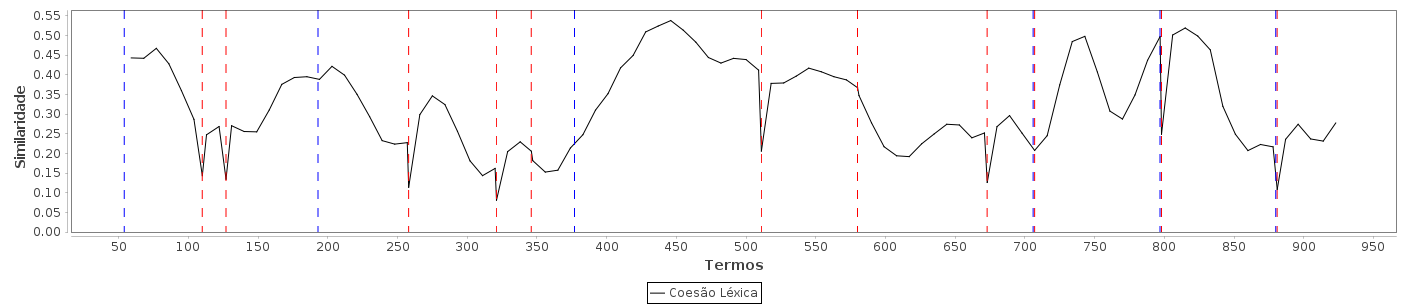
\includegraphics[width=\textwidth]{conteudo/capitulos/figs/coesaolexicaTT-50-9.png}
	  \caption{Variação da coesão léxica ao longo de uma ata junto a uma segmentação automática em contraste com uma segmentação de referência.}
	  \label{fig:coesaolexicaTT}
  \end{figure}


Analisou-se também o desempenho da mesma técnica aplicada a um texto contínuo extraído de artigo da Interent que descreve seis gêneros musicais brasileiros um após um outro separados em seções. Ao observar a Figura~\ref{fig:coesaolexicaTT-generos-musicais}, nota-se que os vales são mais definidos e a maioria dos segmentos coincidem ou estão próximos a segmentação de referência. A segmentação de refência possui sete segementos que separam uma introdução do assuntos e respeitam cada uma das subseções que tratam de um gênero músical.  Obtem-se nesse cenário uma eficiência maior em relação a segmentação da ata, o que sugere que textos organizados em seções podem ter melhores benefícios com técnicas baseadas em coesão léxica que as atas, onde esse fator é menos significativo.  % ou a premissa do algoritmo não é tão boa.



  %--- ---
  \begin{figure}[!h]
	  \centering
	  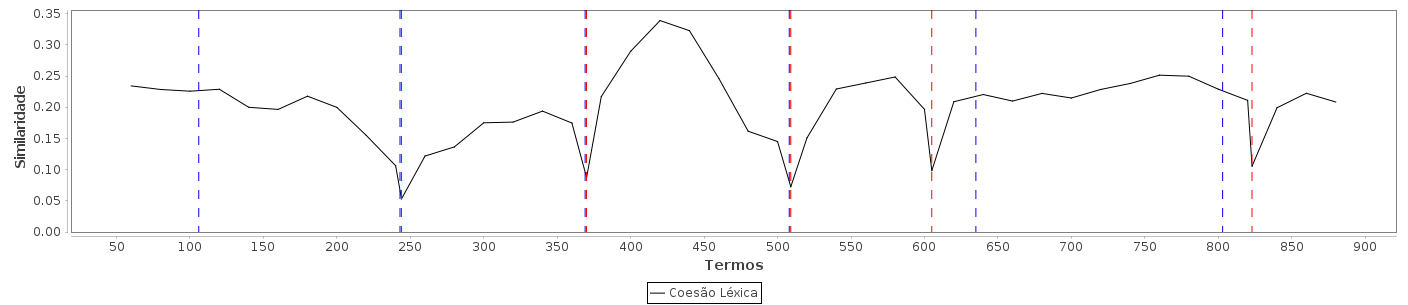
\includegraphics[width=\textwidth]{conteudo/capitulos/figs/generos-musicais-TT-40-20.png}
	  \caption{Variação da coesão léxica ao longo de um artigo melhor estruturado em seções junto a uma segmentação automática em contraste com uma segmentação de referência.}
	  \label{fig:coesaolexicaTT-generos-musicais}
  \end{figure}


  % De certa forma, tratar o C99 e o TT como pertencentes a mesma técnica = coesão léxica!!  % e depois justificar o por que de usar outras técnicas



Na Tabela~\ref{tab:resultadosc99} são apresentadas, as médias obtidas com o \textit{C99} bem como as configurações utilizadas, onde \textbf{S} é a proporção de segmentos em relação a quantidade de candidatos, \textbf{M} é o tamanho do quadro utilizado para criar a matriz de \textit{rankings} e \textbf{W} indica se os segmentos são representados por vetores contendo a frequência ou um peso das palavras.


\begin{table}[!h]
	\centering
	\begin{tabular}{|l||c|c|c|c||c|c|c|c|} \hline

		& \multicolumn{4}{c||}{Sem Pré-processamento} 
		& \multicolumn{4}{c|}{Com Pré-processamento}\\			

		\textbf{Medida} & 
		\textbf{S} & 
		\textbf{M} & 
		\textbf{W} & 
		\textbf{Média} &
		\textbf{S} & 
		\textbf{M} & 
		\textbf{W} & 
		\textbf{Média} \\	\hline

		P$_k$				& 20 & 9 & Sim & 0,134& 20 & 11 & False	& 0,116 \\ \hline  
		\textit{WindowDiff}	& 60 & 9 & Sim & 0,411& 60 &  9 & Sim 	& 0,390 \\ \hline  
		Acurácia			& 60 & 9 & Sim & 0,588& 60 &  9 & Sim 	& 0,609 \\ \hline  
		Precisão			& 40 & 9 & Sim & 0,645& 20 & 11 & False	& 0,720 \\ \hline  
		Revocação			& 80 & 9 & Sim & 0,869& 80 & 11 & Sim 	& 0,897 \\ \hline  
		F$^1$				& 80 & 9 & Sim & 0,638& 80 & 11 & Sim 	& 0,655 \\ \hline  

	\end{tabular}
	\caption{Resultados obtidos com o \textit{C99}}
	\label{tab:resultadosc99}
\end{table}




De acordo com os últimos testes, o algoritmo \textit{C99} obteve melhor desempenho em acurácia, precisão, $F^1$, $P_k$ e \textit{WindowDiff}, enquanto o \textit{TextTiling} obteve o melhor desempenho em revocação como pode ser visto na Tabela~\ref{tab:configfinal}. 







% O algoritmo \textit{C99} obteve melhor desempenho em acurácia, precisão, $F^1$, $P_k$ e \textit{WindowDiff}, enquanto o \textit{TextTiling} obteve o melhor desempenho em revocação como pode ser visto na Tabela~\ref{tab:configfinal}. 


% \begin{table}[!h]
	% \centering

	% \begin{tabular}{|l|l|c|c|c|c|c|} \hline
		% \textbf{Algoritmo} & 
		% \textbf{Medida} & 
		% \textbf{Média}\\	\hline

	% \textit{C99} & P$_k$			   & 0,116 \\ \hline
	% \textit{C99} & \textit{WindowDiff} & 0,390 \\ \hline
	% \textit{C99} & Acurácia			   & 0,609 \\ \hline
	% \textit{C99} & Precisão			   & 0,720 \\ \hline
	% \textit{C99} & F$^1$			   & 0,655 \\ \hline
	% \textit{TextTiling} &	Revocação  & 0,917 \\ \hline

	% \end{tabular}
	
	% \caption{Melhores resultados obtidos.}
	% \label{tab:configfinal}
% \end{table}




\begin{table}[!h]
	\centering
\begin{tabular}{|l||c|c|c|c|c|c|c|} 
\hline 
\textbf{M\'{e}todo} & 
\textbf{Pk} & 
\textbf{WD} & 
\textbf{A } & 
\textbf{P } & 
\textbf{R } & 
\textbf{F1} & 
\textbf{Segmentos}\\ \hline

Senten\c{c}as & 0.320 & 0.502 & 0.498 & 0.498 & \textbf{1.000} & \textbf{0.642} & 22.083\\ \hline
TextTiling    & 0.275 & 0.469 & 0.531 & 0.514 & 0.937 & 0.640 & 19.583\\ \hline
C99           & 0.142 & 0.426 & 0.574 & 0.601 & 0.473 & 0.506 & 8.167\\ \hline
BayesSeg      & 0.148 & 0.414 & 0.586 & 0.599 & 0.526 & 0.528 & 8.750\\ \hline
MinCut        & 0.226 & 0.532 & 0.468 & 0.464 & 0.438 & 0.432 & 10.333\\ \hline
TextSeg       & \textbf{0.085} & \textbf{0.387} & \textbf{0.613} & \textbf{0.714} & 0.412 & 0.497 & 5.167\\ \hline
\end{tabular} 

	\caption{Melhores resultados obtidos.}
	\label{tab:configfinal}
\end{table}









%  we have a winner
Verificou-se que, de maneira geral, o algoritmo \textit{C99} apresenta melhores resultados em relação ao \textit{TextTiling}, contudo, testes estatísticos realizados indicaram que não houve diferença significativa entre os métodos. Nesse trabalho, escolheu-se o algoritmo \textit{C99} por apresentar resultados satisfatórios e ligeira superioridade em relação ao \textit{TextTiling}. 






% cada segmento é um documento
Após a identificação dos segmentos, o algoritmo retorna uma lista onde cada elemento é um texto com um assunto predominante e será a partir de disso considerado um documento.

% -? Medidas

% -- como ele faz?




%  ==========   ==========   ==========   ==========   ==========   

\subsection{Representação Computacional}

As etapas anteriores produzem fragmentos de documentos onde o texto esta em um estágio de processamento inicial, com menos atributos que as versões originais, onde cada fragmento está associado a um tema, porém, ainda não estruturado. Ocorre que as técnicas de mineração de texto exigem uma representação estruturada dos textos. % conforme será visto na Seção~\ref{subsection:RepTextos}.

Uma das formas mais comuns é a representação no formato matricial conhecida como Modelo Espaço Vetorial (\textit{Vectorial Space Model} - VSM)~\cite{Rezende2003}, onde os documentos são representados como vetores em um espaço Euclidiano $t$-dimensional em que cada termo extraído da coleção é representado por um dimensão. Assim, cada componente de um vetor expressa a relação entre os documentos e as palavras. Essa estrutura é conhecida como \textit{document-term matrix} ou matriz documento-termo.  Nesse trabalho a representação empregada é a \textit{Bag Of Words} a qual sintetiza a base de documentos em um contêiner de palavras, ignorando a ordem em que ocorrem, bem como pontuações e outros detalhes, preservando apenas o peso de determinada palavra nos documentos. 



\subsection{Extração de Tópicos}

% a tarefa é identificar qual assunto está presente em cada trecho e qual é o tipo de ocorrência.



\section{Módulo Consulta}

Uma vez que a estrutura de dados interna contem os assuntos abordados na coleção de documentos, o tipo de ocorrência para cada assunto e o trecho onde se encontram, caberá ao módulo de consulta receber a \textit{string} de consulta do usuário, resgatar os dados desejados e apresentá-los em ordem cronológica, dando condições para o usuário acessar os segmentos encontrados bem como os documentos originais.

\subsection{Seleção dos tópicos}

\subsection{Visualização}

O usuário final precisa de uma interface adequada para visualizar os resultados da busca considerando-se a relevância dos tópicos selecionados e a sequência cronológica.

Uma boa apresentação deve permitir ao usuário identificar a relevância os resultados e ser relativante independente para compreensão do conteúdo, evitando a leitura do texto completo. Ou seja, o texto de cada tópico apresentado deve ser suficiente para compreensão do assunto mencionado, sem necessidade de visualizar o documento original.

As informações apresentadas, incluem dados obtidos do documento como o nome do arquivo e data do original e o texto onde o assunto é mencionado. Além disso, apresenta-se as informação extraídas pelas técnicas de mineração de texto como os descritores e rótulos.

% o sistema traz vários resultados para uma consulta, alguns mais relevantes que outros. Para cada resultado (que podem tratar de coisas diferentes) o sistema apresenta um histórico de menções para aquele assunto;

Para cada busca, é retornada uma lista de resultados ordenados pela relevância com a \textit{string} de entrada, sendo cada item referente a uma menção a um assunto. Um tópico é abordado em diferentes momentos e registrado em atas distintas, onde cada menção é um resultado a ser apresentado. 

Como parte da proposta, o sistema apresenta cada resultado dentro de um histórico de menções. Para isso, abaixo do texto é exibida uma linha com links para os resultados que compartilham o mesmo tópico ordenados por data. Os links, ao ser acionado, direciona para o resultado que aponta, além disso, quando o cursor do mouse está sobre o link, é apresentado um pre-visualização do texto. Dessa forma o usuário tem acesso uma interface que lhe fornece uma visão temporal das menções.

% Uma vez que um item faz menção a um tópico específico, 


% um histórico de menções para o assunto pesquisado.
% O sistema também apresenta junto com cada resultado, 


\section{Estudo de caso}
% -- qual o ganho em relação a um sitema de busca por palavras-chave? 


\section{Avaliação}

